\documentclass[english]{upeeei}
\usepackage[latin9]{inputenc}
\setcounter{secnumdepth}{3}
\setcounter{tocdepth}{3}
\usepackage[active]{srcltx}
\usepackage{units}
\usepackage{parskip}
\usepackage{graphicx}
\usepackage{subfigure} 
\usepackage{url}  
%\usepackage{stfloats}  
\usepackage{amsmath}   
\usepackage{array}
\usepackage{caption}
\usepackage{afterpage}
\usepackage{textcomp}
\usepackage{lscape}
\usepackage{stfloats}
\usepackage{hyphenat}
\usepackage{makeidx}
\usepackage{amssymb}
%\usepackage{underscore}
\fnbelowfloat
\usepackage{times}
\usepackage{multirow}
%\usepackage{float}
\usepackage{circuitikz}
\usepackage[backend=bibtex,bibstyle=ieee,citestyle=numeric-comp]{biblatex}
\addbibresource{Proposal_Part1.bib}
\usepackage{pgfplots}
%\usepackage{arydshln}
\pgfplotsset{width=7cm,compat=1.5.1}
\renewcommand*{\bibfont}{\small}

\newcolumntype{L}[1]{>{\raggedright\let\newline\\\arraybackslash\hspace{0pt}}m{#1}}
\newcolumntype{C}[1]{>{\centering\let\newline\\\arraybackslash\hspace{0pt}}m{#1}}
\newcolumntype{R}[1]{>{\raggedleft\let\newline\\\arraybackslash\hspace{0pt}}m{#1}}

\newcommand\ddfrac[2]{\frac{\displaystyle #1}{\displaystyle #2}}
\pgfplotsset{compat=1.14}

\makeatletter

%%%%%%%%%%%%%%%%%%%%%%%%%%%%%% LyX specific LaTeX commands.
\providecommand{\LyX}{L\kern-.1667em\lower.25em\hbox{Y}\kern-.125emX\@}
%% Because html converters don't know tabularnewline
\providecommand{\tabularnewline}{\\}

\@ifundefined{showcaptionsetup}{}{%
 \PassOptionsToPackage{caption=false}{subfig}}
\usepackage{subfig}
\makeatother

\usepackage{babel}

\begin{document}
%%% UP EEEI undergraduate project template
%% v0.1 by Louis P. Alarcon 11/22/2011
%%
%% LyX template - use with the following files:
%% 	uct10_new.clo, uct11_new.clo, uct12_new.clo, upeeei.cls, upeeei.layout
%%
%% Place project title here
\title{Autonomous 3D Indoor Mapping Using Unmanned Aerial Vehicles} 

%%
%% Author information

\author{
%% Use \vspace to separate each member
%% Put your names here in alphabetical order
\\Louie Isaniel Cachola Henson \\ 2014-30227 \\ \emph{B.S. Computer Engineering}
}

%%
%% Month and year of submission/graduation
\degreeyear{2021} 
\degreesemester{January} 

% Put your advisers here:
\chair{Professor Charleston Dale Ambatali
\\
Professor Roxanne De Leon
} 
%\othermembers{John Richard Ereso Hizon\\ 
%Joel Joseph Sarco Marciano, Jr.} 
\numberofmembers{1} 

\field{Electrical/Computer/Electronics and Communications Engineering} 
\campus{Diliman} 

\maketitle
% \approvalpage 
% \copyrightpage 
\begin{abstract} 

%Your abstract goes here...
\textbf{Multirotor unmanned aerial vehicles} (or drones as they are more commonly known) are quick and versatile, often 
proving to be a great asset for survey or reconnaissance missions. However, learning to pilot a UAV can prove to be 
difficult and expensive. The goal of this project is to develop a drone that can not only provide the user with an
accurate 3D map of indoor spaces but do so \emph{autonomously}. This would require a robust flight controller capable of
accurate simultaneous localization and mapping (SLAM) and efficient 3D navigation and exploration. Performance of the UAV
will be assessed in terms of exploration speed and mapping precision.

\end{abstract}

\begin{frontmatter}
\setlength{\parskip}{0pt}
\tableofcontents
\listoftables
\listoffigures
\end{frontmatter}
\def\MASTERDOC{true}

\chapter{Introduction}
As technology develops, unmanned aerial vehicles continue to be integrated into increasingly diverse environments and
fields. From photography and cinematography, all the way to military applications. Similarly, 3D mapping has found uses
in fields such as archaeology and architecture, all the way to disaster risk reduction and management. They are especially
useful for reducing the amount of risk that personnel experience by flying to places that pose a significant hazard to 
the personnel. This necessitates the development of more complex ways of controlling the UAV that would effectively 
lower the learning curve that new pilots have to face. Autonomous functions also lower the risk of human error by 
limiting the amount of ways that the pilot can influence the actual flight. The development of a flight controller 
system capable of autonomous 3D indoor mapping can be divided into the development of several components; the flight 
controller board, the SLAM (simultaneous localization and mapping) algorithm, the autonomous exploration function, and 
the mobile radio controller that allows the pilot to interface with the UAV.
\section{Flight Controller Design}
The flight controller is, as its name suggests, the central device that controls how the UAV moves and reacts to certain
stimuli. The flight controller contains multiple sensors including (but not limited to) a gyroscope, accelerometer, and
barometer. These sensors allow the flight controller to get a sense of its orientation in 3D space. The flight controller 
will also be responsible for communicating with a base station and processing commands correctly. In order to make the
UAV easy to mass produce and more affordable, production cost was prioritized while designing the flight controller.
Several methods for designing the flight controller were found but one was seen to be the most cost-effective and
flexible solution. Establishing a well functioning flight controller is important as it is essentially the cornerstone of the
UAV and will influence work on both the autonomous navigation functions as well as the simultaneous localization and
mapping (SLAM) functions.
\section{Simultaneous Localization and Mapping}
Simultaneous localization and mapping (SLAM) is the process where a machine maps out its immediate environment and gets
a sense of where it is in that environment. This is especially useful for autonomous exploration as it allows the UAV to
formulate an obstacle-free trajectory to its target. Mapping often makes use of a lidar sensor
\cite{Dowling2018} or one or more cameras\cite{OrbSlam2} depending on the level of accuracy and speed that is required. 
\section{Autonomous Navigation}
Autonomous navigation is the process where a machine navigates to a target location while avoiding obstacles. This is
often used in tandem with SLAM and path finding algorithms such as Dijkstra's algorithm or even neural networks 
\cite{Dowling2018}. Methods of navigation include global and local navigation however \cite{Dowling2018} notes that the
best results can be foound by combining the two.

\chapter{Review of Related Work}
\section{Flight Controller Board Design}
As building a flight controller from scratch would prove to be akin to reinventing the wheel, a premade flight controller
will be used as a base that this project will build upon. The base flight controller will be responsible for communicating
with the electronic speed controllers (ESCs) and controlling the motors on a more basic level. \cite{MultiwiiFC} shows how
to build a basic flight controller. The corresponding diagram for the system is represented by figure
\ref{fig:base_FC_diagram}. The flight controller makes use of a microcontroller that is connected to an inertial
measurement unit (IMU). The IMU includes an accelerometer and gyroscope that allow the flight controller to discern its 
orientation in 3-dimensional space. Based on these readings, the flight controller will update the ESCs with the proper
outputs.Based on figure \ref{fig:base_FC_diagram}, we will essentially be treating the base flight controller as a black
box. The inputs, as seen with \cite{MultiwiiFC} would be a PPM signal containing the throttle, yaw, pitch, and roll signals.
The Pixhawk, another family of flight controllers as demonstrated by \cite{RPiMavlink2019} make use of MAVLink (Micro Air
Vehicle Communication Protocol) to deliver the necessary signals into the flight controller. MAVLink makes use of a UART
connection to send instructions to the flight controller. \cite{RPiMavlink2019} makes use of a Raspberry Pi to communicate
with the Pixhawk. This allows them to interface with the UAV in a more sophisticated manner and make use of the computer's
higher processing power. \cite{Redtail2017} demonstrates how to use an onboard computer to apply neural networks for
intelligent flight control. Meanwhile, \cite{Dowling2018} uses a Raspberry Pi coupled with a lidar sensor to allow the UAV
to autonomously navigate and map out its surroundings on a 2D plane. This is shown in figure \ref{fig:FC_system_diagram}.
\begin{figure}[h]
    \centering
    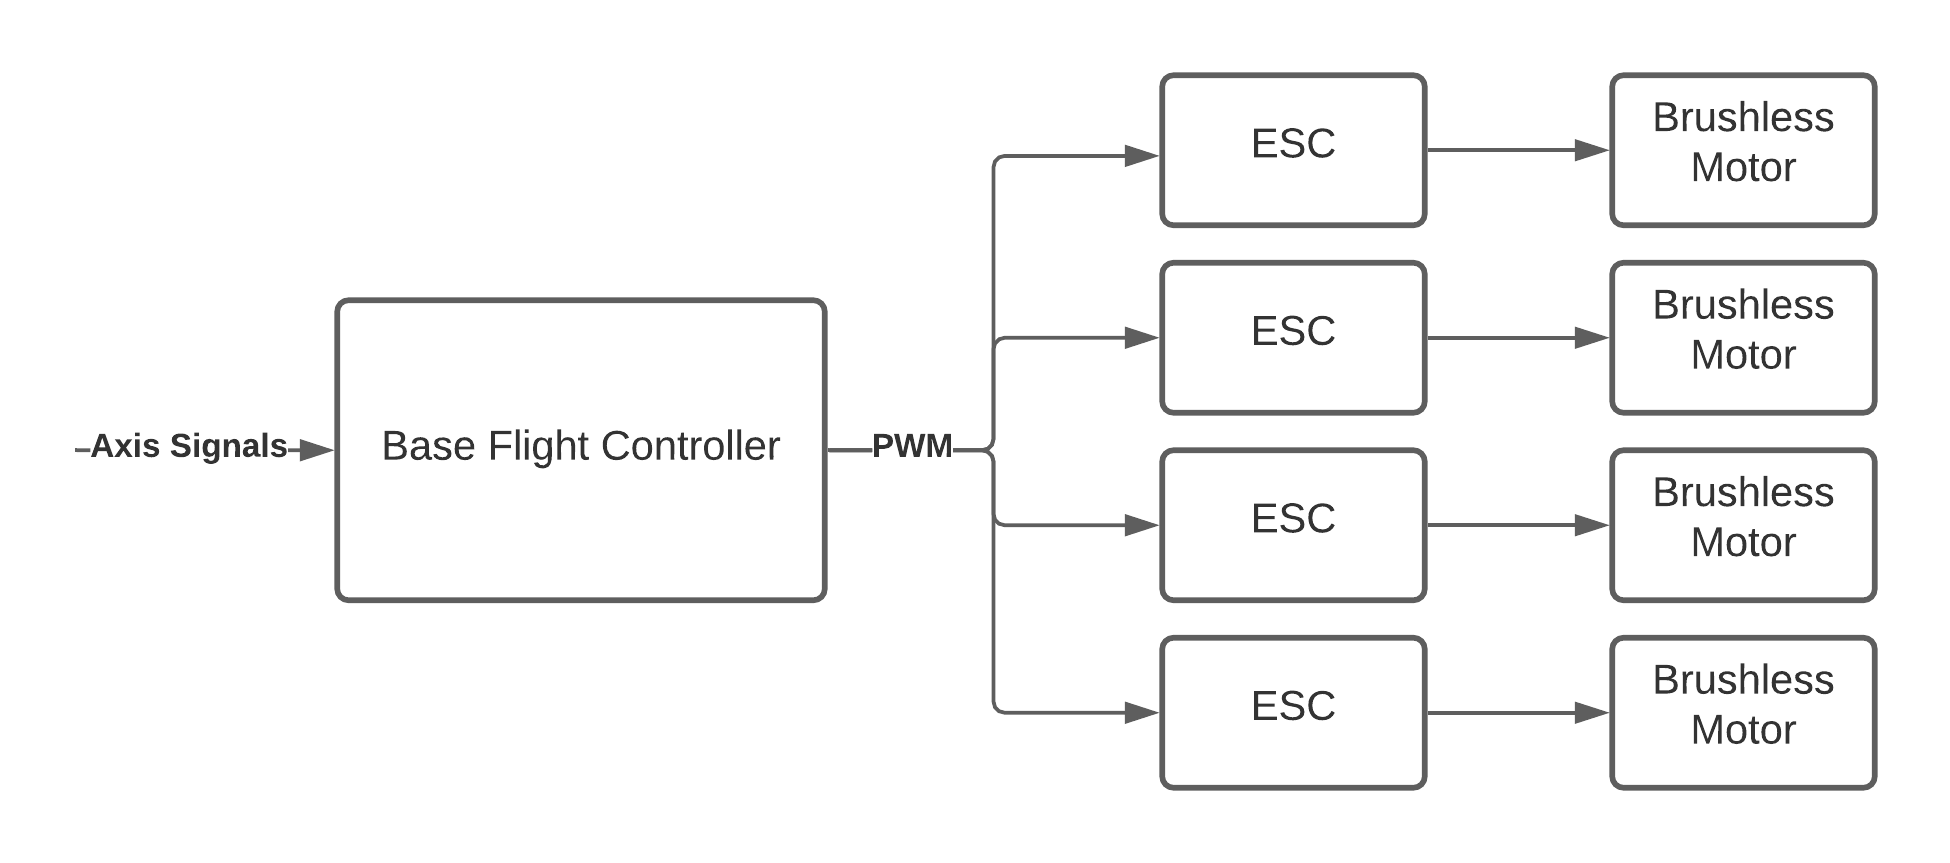
\includegraphics[scale=0.5]{images/base_FC_diagram.png}
    \caption{Diagram of base flight controller connected to ESCs and motors}
    \label{fig:base_FC_diagram}
\end{figure}
\begin{figure}[h]
    \centering
    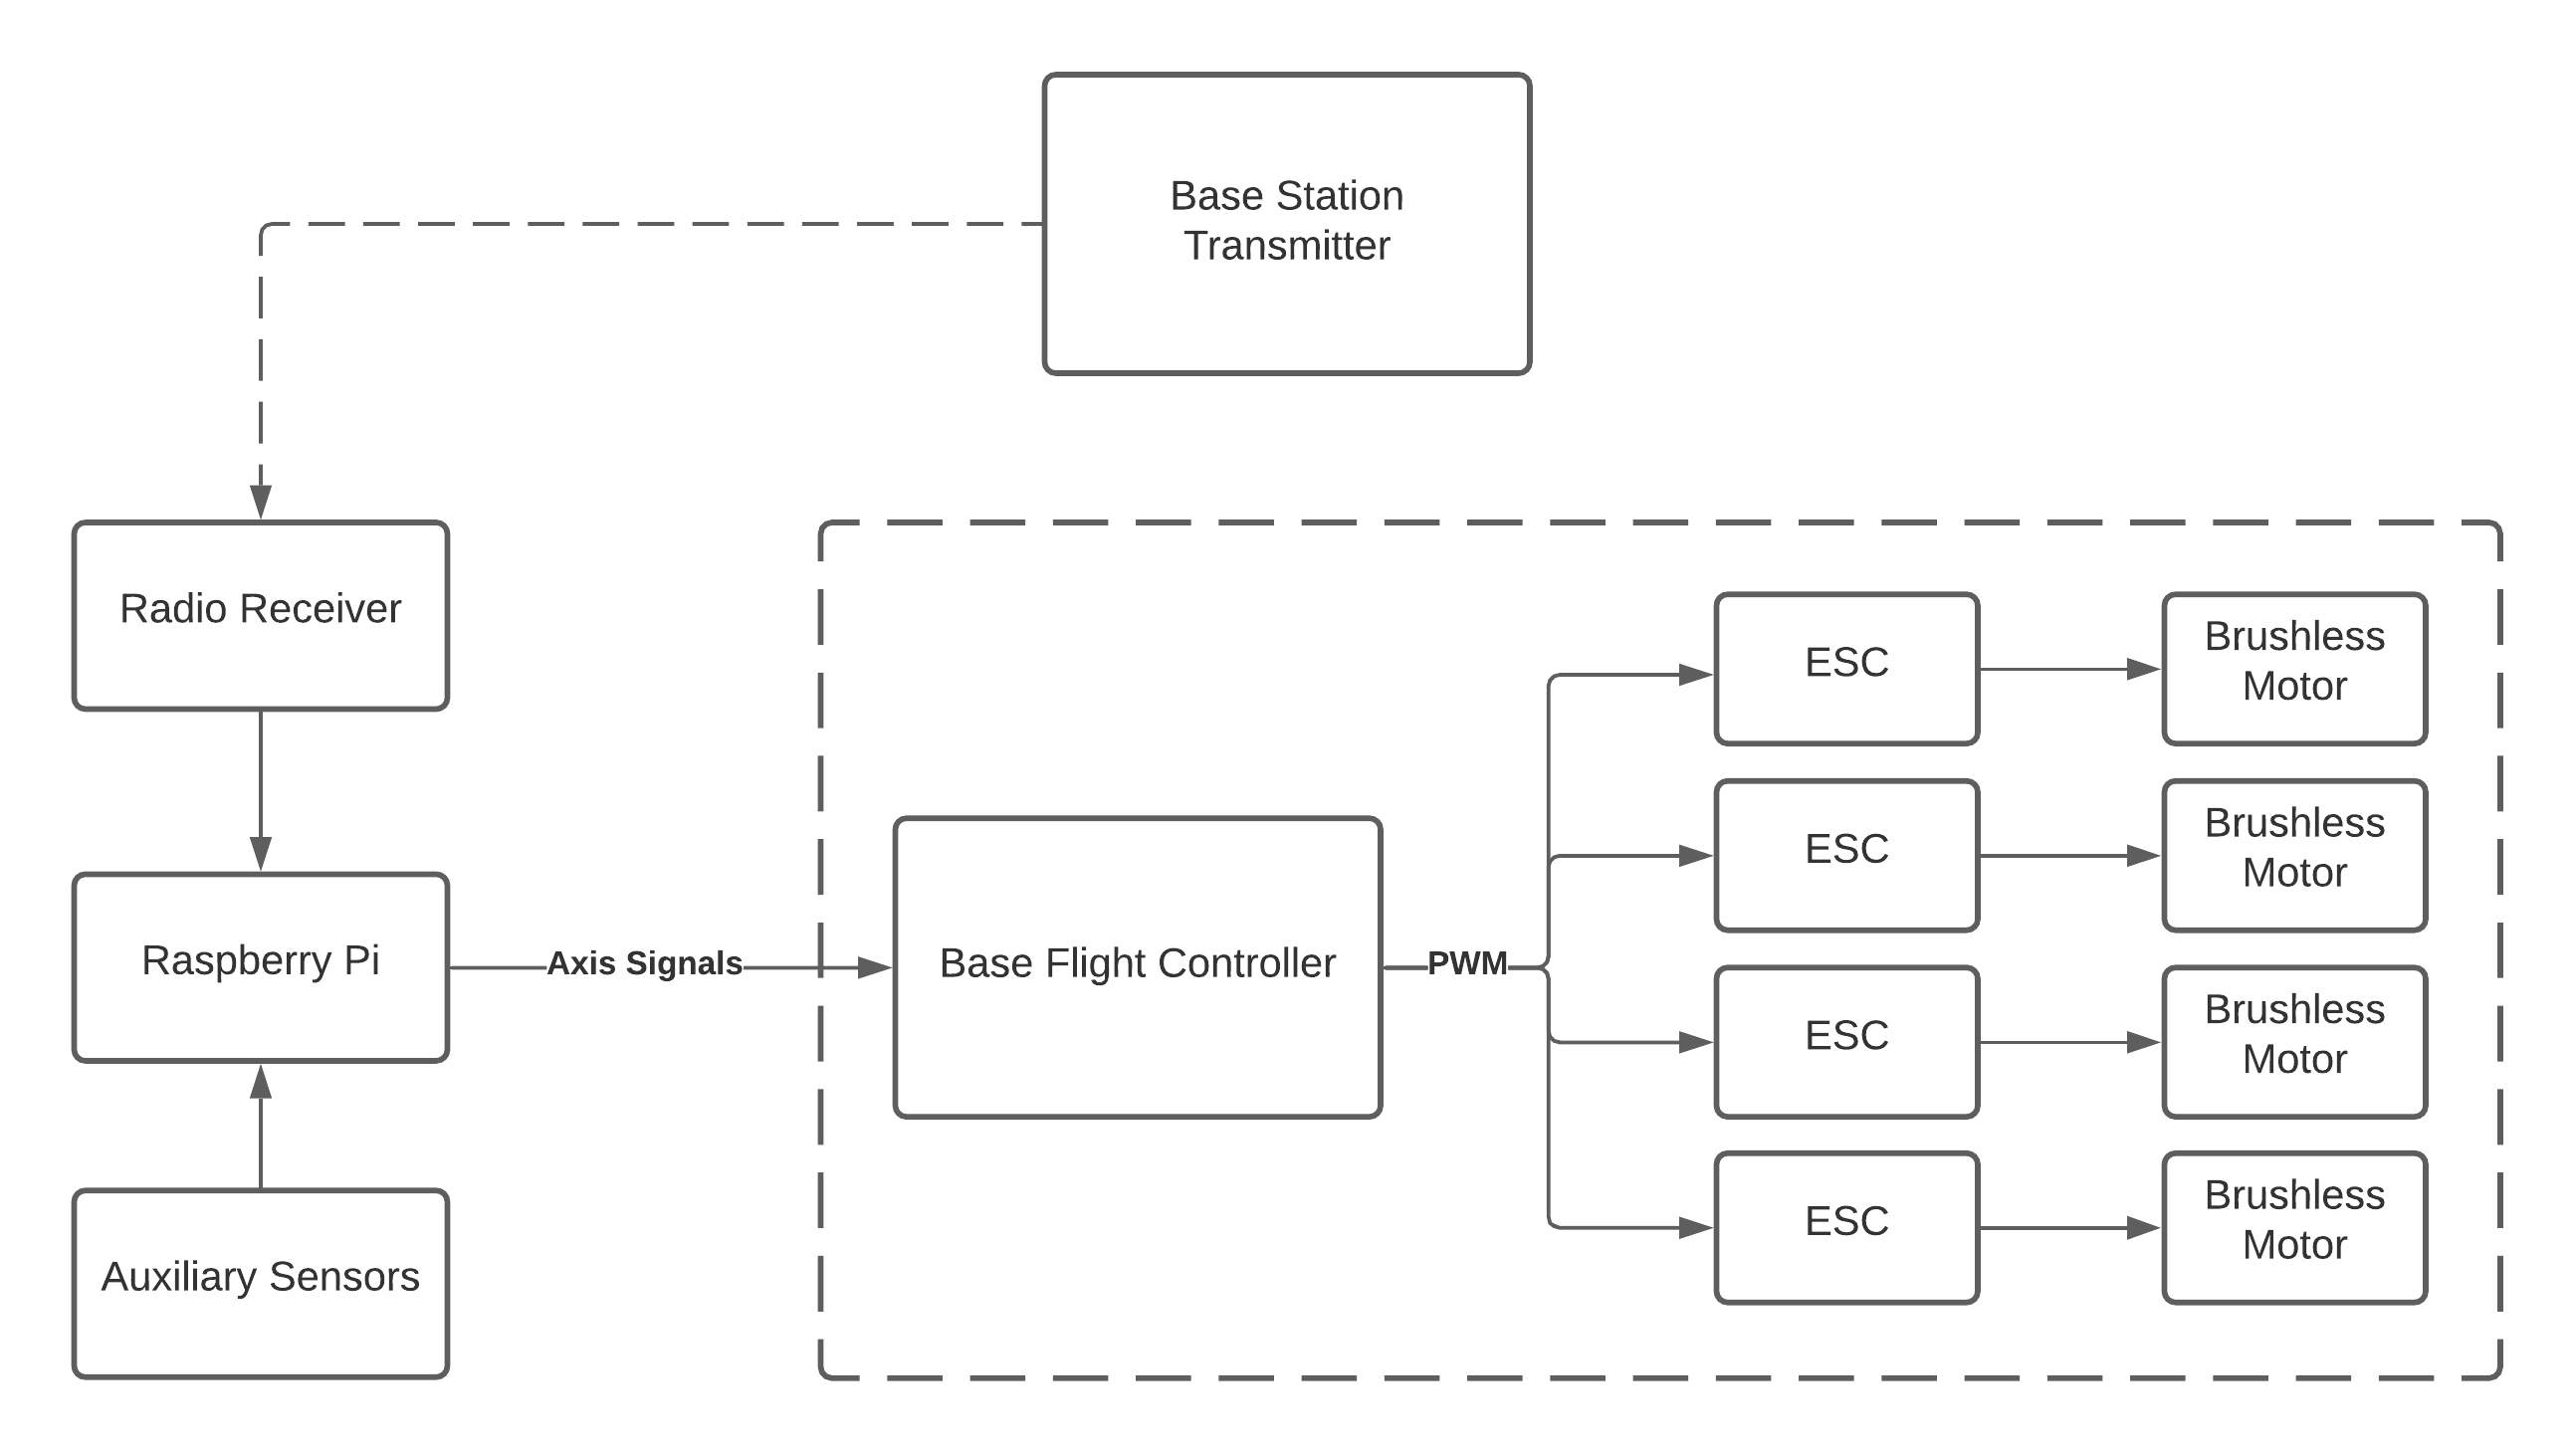
\includegraphics[scale=0.5]{images/fc_with_rpi.png}
    \caption{Diagram of flight controller system with raspberry pi}
    \label{fig:FC_system_diagram}
\end{figure}
The base flight controller itself is a PID controller. The firmware allows us to manually tune the PID values depending 
on the user's preference. \cite{Tuning2017} demonstrates a more robust way of tuning the PID values as compared to the
more traditional heuristic methods.
\section{Simultaneous Localization and Mapping}
An open-source SLAM API was proven to be functional in \cite{OrbSlam1}. The API makes use of a monocular camera as an
input device and is able to reconstruct both indoor and outdoor environments in real time. This SLAM system was developed
with ground based robots and cars in mind. It essentially works by selecting a number of points of interest in one frame
of the video then matching these points to similar points of interest in the next frame. It then takes the difference in
position of these point of interest and calculates depth from there. The authors then further improved the accuracy in
\cite{OrbSlam2}. Here, they expanded the input to stereo cameras and depth cameras as these seemed to provide much more
accurate results. The authors found that using only a monocular camera was prone to failures as more rotations were used
in the machine's exploration. They also found that using multiple cameras (as in the stereo camera) significantly
improved the accuracy of depth perception. Another aspect that the authors improved upon is the fact that this version
was developed to be an out-of-the-box SLAM solution. As a result, this version provides more support for varying systems
and is much easier to use as compared to the previous version. However this version does have its lapses where processing
power is concerned. Due to the heavy operations being performed, it would struggle to perform even on a Raspberry Pi 4. 
Looking for a lightweight SLAM solution, \cite{FastSlam2} presents a SLAM system for low-power embedded architectures,
which would be more ideal for the purposes of this project. The authors used a 320x300 resolution camera connected to a
Raspberry Pi 2B. While the system was able to function within the low-power specifications, it suffers in terms of
accuracy. The system was significantly less accurate than the SLAM systems seen in \cite{OrbSlam1} and \cite{OrbSlam2}.
The authors claim that this was due to the low resolution of the camera used and that accuracy can be further improved
by using an encoder with a higher resolution. Finally, \cite{SVO2017} presents a lightweight but accurate solution for
localization and mapping. \cite{SVO2017} makes use of semi-direct visual odometry (SVO). Primarily developed for use with
UAVs and monocular cameras, SVO boasts a reduction in CPU usage of up to 79.45\% compared to \cite{OrbSlam2}. SVO is also
up to 11.8 times faster while maintaining an accuracy that is 13.5 times better than that of \cite{OrbSlam2}. SVO does 
away with feature extraction and matching procedures by estimating the movement of the camera system using the pixel
intensities per frame.
\section{Autonomous Navigation}
Autonomous navigation consists of two methods; global and local. Global navigation methods involve planning out the general
trajectory of the robot without taking into account the local movement restriction of the robot. This entails planning out
the overall path that the robot will take when reaching its goal. By contrast, local navigation methods involve planning
the trajectory of the robot around its direct environment. This involves more minute movements and obstacle avoidance. 
According to \cite{Dowling2018}, the best navigation results have been obtained by combining both of these methods. The
navigation system used by \cite{Dowling2018} mimics navigation systems used by ground based robots and adapts them to suit
UAVs flying at a fixed height. Their system simulates all possible trajectories that the UAV can take and assigns a cost
to each one. The UAV then takes the path with the smallest cost. While this method functions well for 2D mapping and
navigation, this would be lacking for this project as we would need to navigate in 3D. Luckily, \cite{Fuel2020} presents
a method for performing fast UAV exploration in complex environments (FUEL). It starts similarly by finding the most optimal
global trajectory that is available to the UAV. It then continually recalculates as more and more regions are explored.
FUEL is based on the frontier method of navigation where the UAV looks for the nearest unexplored region. The authors also
introduce a frontier information structure (FIS) that contains information on the environment. The structure is then updated
continuously and allows for high frequency planning. Based on the FIS, the system then generates a heirarchy of motions
in three steps (course to fine). The heirarchical planner finds efficient global paths, selects a local set of optimal
viewpoints, and from there, generates the best trajectory based on the minimum time. Alternatively, \cite{ProbNav}
presents a different method of navigation that deviates from the frontier method and instead adopts a method based on
incremental sampling and a probabilistic roadmap. In this method, nodes are incrementally added to the explored regions to
generate the best viewpoints for the camera system. These viewpoints are those that provide the system with the most data
points, thereby mapping the most amount of regions in the least time. The probabilistic roadmap allows for rapid searching
of alternative global and local paths that the UAV can take. However the authors found that the system was not able to
locate all obstacles 100\% of the time, raising concerns with regards to the safety of the UAV while navigating.
\chapter{Problem Statement and Objectives}

This project aims to develop a low-cost UAV capable of autonomous 3D indoor mapping. 
\chapter{Methodology}
This project can be divided into three milestones; flight controller design and fabrication, integration of SLAM, and
finally, integration of autonomous navigation system.
\section{Flight Controller Design and Fabrication}
Cost, size, and weight will be the primary deciding factors for the flight controller design. For the base flight
controller, the MultiWii will be implemented as demonstrated by \cite{MultiwiiFC}. This allows for a much more flexible
and cost effective solution. The microcontroller to be used will be the Arduino Pro Mini, which provides a small
footprint. It will then be wired to send pwm signals to a 4-in-1 ESC board. A 4-in-1 ESC board was selected over
individual ESC modules because the board is lighter, smaller, and is less costly. Furthermore, less wiring will need to
be done, leading to easier mass production. The motors will be 2400KV brushless motors suitable for 5 inch propellers.
For the inertial measurement unit, the MultiWii will be connected to an MPU6050 via an I2C interface. The MPU6050 includes
both an accelerometer and a gyroscope. The arduino will be receiving instructions from a Raspberry Pi 4. There are two
options for communication between the Raspberry Pi and the Arduino; single wire PPM and PWM over multiple wires. Both
methods will be tested to find the method with the most stable signal. The Raspberry Pi will also be receiving data from
a GY-87 module, which contains an accelerometer, gyroscope, barometer, and magnetometer which are all accessible via
I2C protocol. This will aid the UAV with regards to SLAM and navigation. Aside from this, the Raspberry Pi will also be
connected to a GPS module which, while inoperable during indoor operations, will prove to be essential during outdoor
missions especially when locating the UAV. For communication, the flight controller will be employing a LoRa RA-02 module,
which was chosen for its long range capabilities. The LoRa module will be communicating with a similar module connected to
the base station. A diagram of the system may be seen in figure \ref{fig:final_FC_diagram}. The goal of this milestone is
to design and fabricate a Raspberry Pi hat that contains all the necessary components of the flight controller.
\begin{figure}[h]
    \centering
    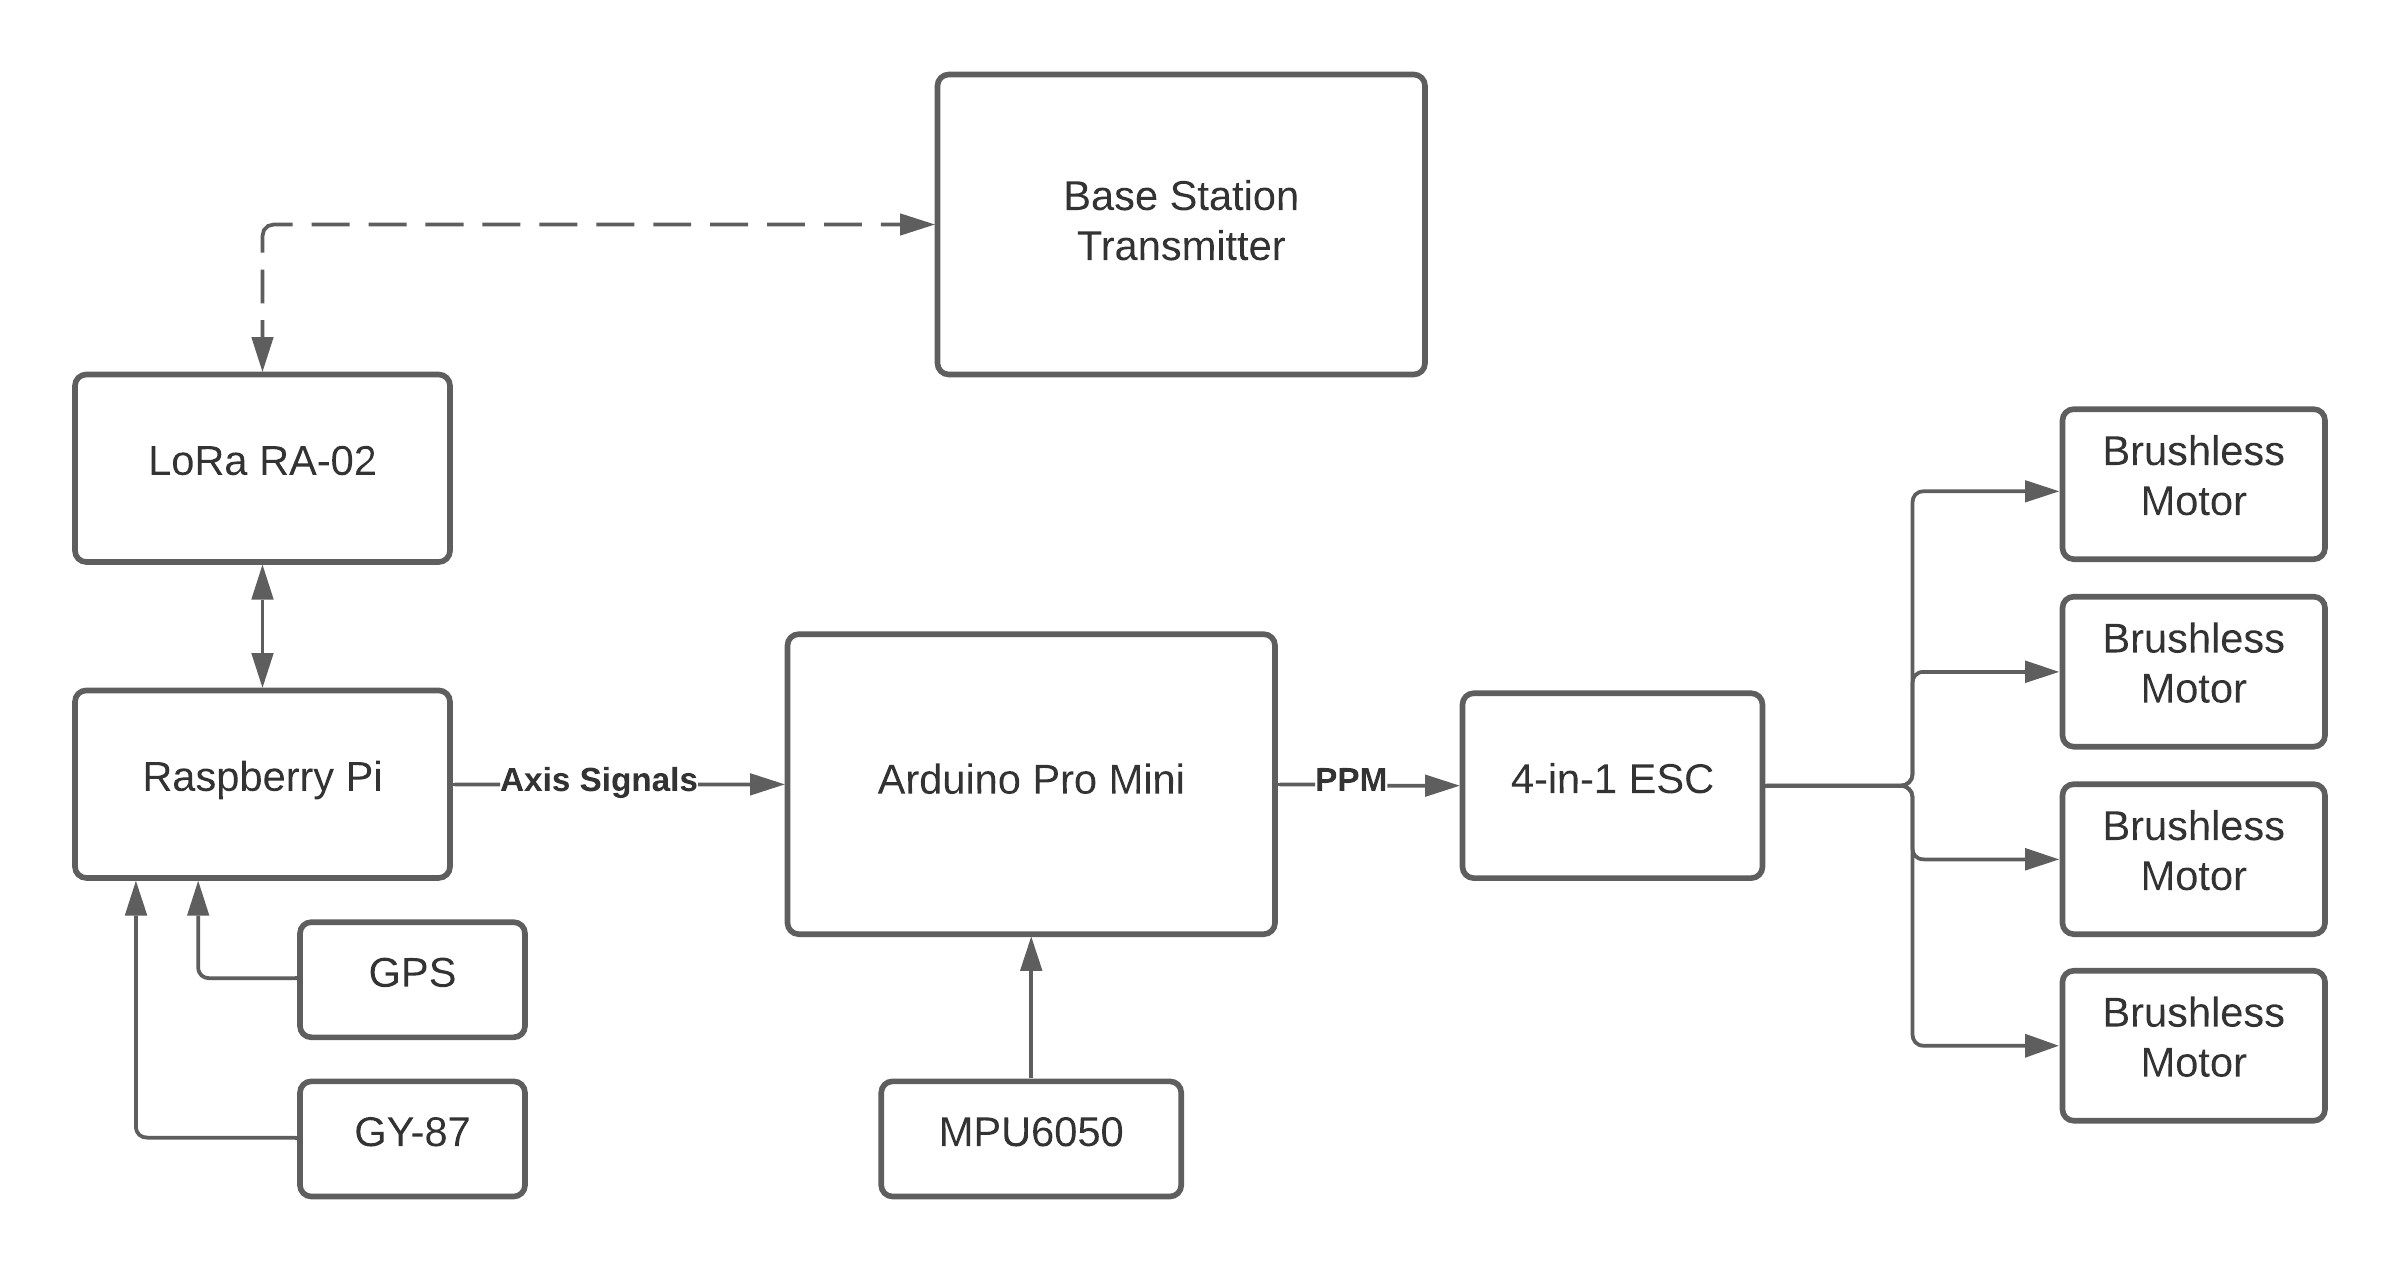
\includegraphics[scale=0.5]{images/final_FC diagram.png}
    \caption{Flight controller diagram with ESC module and motors}
    \label{fig:final_FC_diagram}
\end{figure}
\newline
\newline
The Raspberry Pi will be running the latest version of Raspbian. It will then be using ROS (robot operating system) for
the UAV's processes. ROS is an open source robotics framework that was designed to be modular and flexible, taking into
account the multitude of processes that a robot needs to run. In the case of this project, the modularity allows for
easier integration of different modules and functions. This in turn means that the source code will be easier to maintain
as more and more functions are added.
\newline
\newline
Once the flight controller has been assembled, it then needs to be calibrated and tuned. Fortunately, the MultiWii also
comes with a GUI that allows users to calibrate and tune the sensors and PID values. The gyroscope and accelerometer may
be calibrated automatically via the GUI however the PID values must be calibrated manually. Typical heuristic methods
involve test flights where a pilot performs sharp maneuvers in order to see how the UAV reacts. They then come back to the
interface and adjust the PID values based on trial and error. Fortunately, \cite{Tuning2017} provides a more robust method
of tuning. After calibration and tuning, the UAV should function similarly to an off-the-shelf quadcopter.
\section{SLAM Integration}
There are two outstanding choices for SLAM; Orb SLAM 2 \cite{OrbSlam2} and SVO \cite{SVO2017}. Orb SLAM 2 provides a
powerful and fast out-of-the-box solution for SLAM however due to the processing power restrictions, SVO proves to be the
more ideal system. Luckily, the developers have already provided a means to integrate SVO into the ROS framework.
Therefore, applying SVO to the UAV should be a trivial matter. Data from SVO will then be communicated via the RA-02
module back to the base station so that the pilot may have a real-time view of how the mapping operation is progressing.
\section{Autonomous Navigation and Exploration}

\chapter{Timeline}
\section{Gantt Chart}
\section{Halfway Deliverables}

\printbibliography[
heading=bibintoc,
title={Bibliography}
]

\end{document}